\subsection{Время рендеринга}

Результаты измерения времени рендеринга изображены на \ref{fig:perfomance}.

\begin{figure}[h!]
    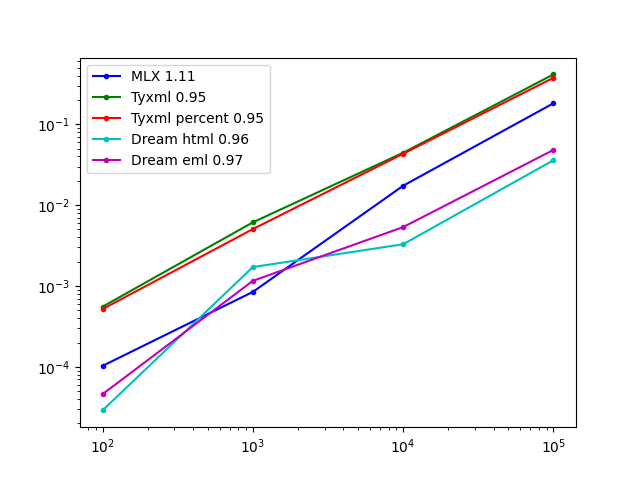
\includegraphics[width=\textwidth]{perfomance.png}
    \caption{Сравнение производительности шаблонизаторов. График построен с помощью пакета matplotlib. Числа в легенде соответствуют аппроксиммированному углу наклона прямых. Масштаб выбран логарифмическим для удобства. Доополнительные детали анализа можно также найти в \ref{apx:tyxml_performance}}
    \label{fig:perfomance}
\end{figure}

EML показал средний результат в сравнении с остальными шаблонизаторами.

По показателям выделения памяти, выдвинута гипотеза о том, что проблема в чрезмерном количестве аллокаций.


